\documentclass[12pt]{article}
\usepackage{amsmath}
\usepackage{graphicx}
\usepackage{hyperref}
\usepackage[latin1]{inputenc}
\usepackage{nopageno}
\usepackage{fancyhdr}
\pagestyle{fancy}
\pdfpageheight=11in
\pdfpagewidth=8.5in

\title{Exchange-Traded Neural Network}
\author{Echometer Rain}
\date{03/12/2024}
\cfoot{This work is licensed under a "CC BY 4.0" license.}

\begin{document}
\maketitle

\begin{abstract}
  We propose a novel financial instrument that replicates the structure of a deep neural network by using exchange-traded funds (ETFs) as perceptrons and options contracts as activation functions. Although legislatively improbable, we predict that such an architecture will be capable of learning time-independent patterns within the stock market (and make us bloody rich) if implemented.
\end{abstract}
\section{Introduction}
Although time-series stock forecasting remains a popular subfield within the study of artificial intelligence, none yet have been unhinged enough to construct a physical neural network using existing financial instruments. This paper details how such technology may be created.
\section{Architecture}
Neural networks are built by passing numerical inputs into a layer of nodes (perceptrons). Each node multiplies its inputs by its corresponding weights and passes the sum of products (typically implemented using a dot product) into an activation function. This process is repeated by passing the outputs of each layer as inputs to the next until a final layer generates an interpretable result. By the Universal Approximation Theorem (UAT), this structure is capable of approximating any mathematical function to arbitrary precision. \newline

To physically reproduce this on the stock market, we notice that the profit function of an options contract is simply a transformed Rectified Linear Unit (ReLU), a widely used activation function. Through this, an Exchange-Traded Fund (ETF) can effectively replicate the workings of a perceptron by buying a certain number of options corresponding to the weight of each input and returning their earnings to the next layer of ETFs.

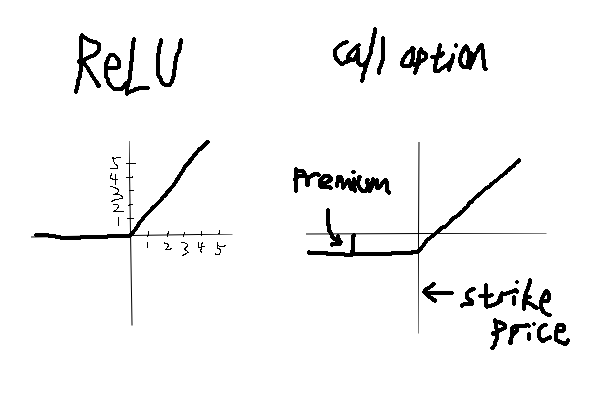
\includegraphics[scale=0.8]{./relu.png}

Let's walk through the transactions to see how such a network would operate: First, the weights of each node are randomly assigned. The input layer of ETFs then buys the amount of options contracts specified by their weights (rounded to integers). The ETF will buy call options if the sign of the weight is positive and it will buy put options if it is negative. After all options are bought, the ETF will start selling options of itself to successive layers. These ETF options will expire when all of the contracts bought by the input layer expire. The process of buying and selling options is repeated until the final layer, the profits of which should be representative of the profits of the entire network.

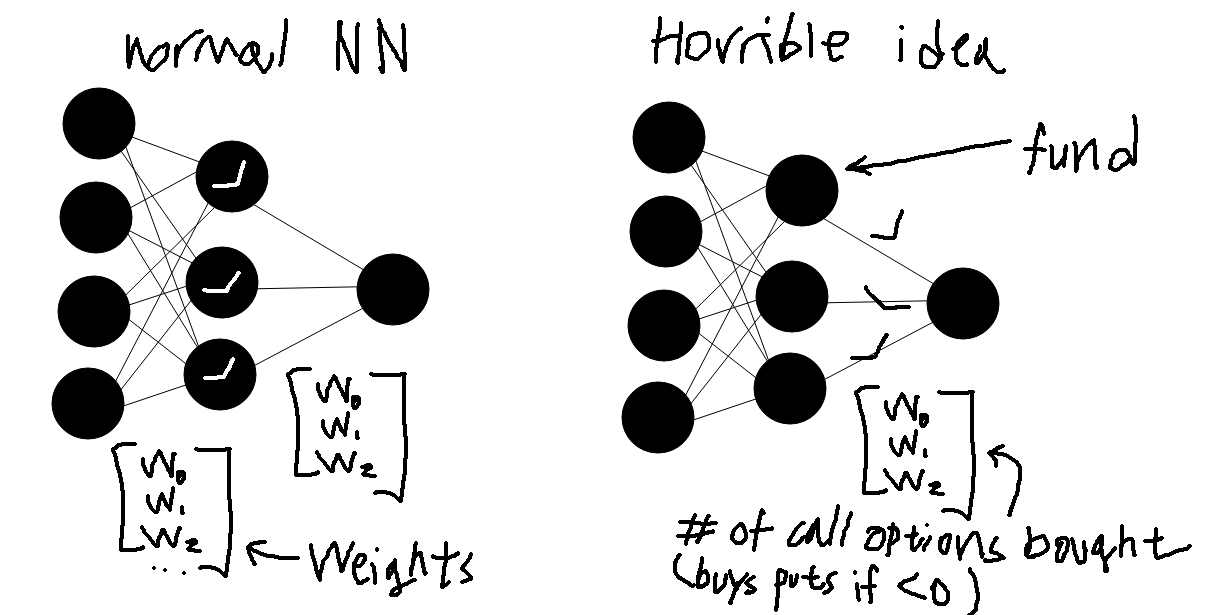
\includegraphics[scale=0.4]{./network.png}
\linebreak

We have not yet implemented the bias term needed to satisfy the Universal Approximation Theorem as treating this will require special considerations. A new bias ETF will be created which buys and sells extremely low volatility stocks according to a random table. Every time the network is activated, the price of the ETF will change by a specific amount. The nodes of the network which depend on the bias will always know whether its price will rise or drop, and they can use this to generate a predictable stream of income. Because no sane investor would want to bet their money on a stepwise random walk (not all investors are sane), the operators of the network would need to sell options to it at a loss whenever it activates. To prevent the network from reward hacking the operators' money away, all profits gained via the bias ETF will be deducted within the loss function.
\linebreak

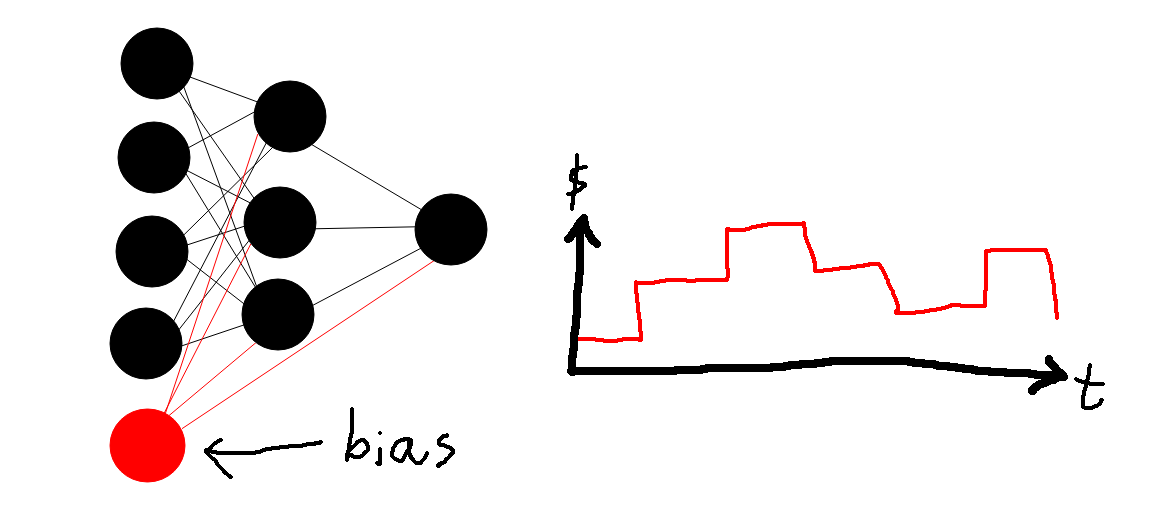
\includegraphics[scale=0.4]{./bias.png}

This brings us to the backpropagation step. To tune the weights of a traditional neural network, a differentiable loss function in order required to measure the amount that each weight of each node contributes to the quality of the final result. In our case, the loss function will just be the net profit of the network, which will equal the net profit of the output layer minus the sum of all the bias weights and the sum of all transaction fees. At the end of each epoch (the time of which depends on the length of the longest contract), the weights can be adjusted to maximize profit, and the network shall run again.
\section{Conclusion}
Not only is this architecture incredibly expensive to train, the Security and Exchange Commission (SEC) will never allow some startup to create $\sim$7000 ETFs out of thin air (without bribes). Because we may not be able to control whether or not an LLM will overfit past stock market data, we predict that our architecture will surpass the investment capabilities of near-future GPTs. We hereby request eight (8) trillion dollar.

\end{document}
